\chapter{Analyse des annotations, explicabilité des modèles autour de la frustrations}
\label{chapitre7}

\section{Motivations}
Lors de cette thèse, nous avons établi des systèmes de reconnaissance continue de l'émotion qui permettent de détecter la satisfaction et la frustration avec un degré d'erreur acceptable.
Dans ce dernier chapitre, nous avons voulu questionner la stratégie qui consiste à fusionner les annotations individuelles de chaque annotateur.
Ainsi nous souhaitons proposer une alternative à la conception la plus établie en matière d'annotation en émotion.
Dans un second temps, la modalité linguistique étant celle qui induit les meilleures performances, il nous semblait important d'essayer de comprendre la prévalence de cette modalité.

Dans la littérature, on a pour habitude d'utiliser de nombreux annotateurs et de fusionner les annotations pour atténuer le caractère subjectif d'une annotation. En effet, il est difficile de nier que la reconnaissance d'une émotion et de son intensité peut varier en fonction de la personne qui la perçoit et en fonction du moment pour une même personne. Il est donc possible d'avoir autant de versions différentes d'a'nnotations que d'annotateurs. Dans ce cas, ne peut-on pas considérer que chaque annotateur est dans le juste ? Nous analysons ce positionnement dans la prochaine section.

Comme nous l'avons établi dans le précédent chapitre, nous pouvons observer que la modalité linguistique permet d'atteindre les meilleurs scores de reconnaissance continue des émotions de satisfaction et de frustration contenues dans AlloSat. Nous aurions pensé dans un premier temps que la modalité acoustique donnerait de meilleurs résultats. En effet, la modalité acoustique, telle que nous la traitons, contient déjà les informations linguistiques. Elles ne sont pas extraites et pré-traitées mais nous pensions que le système de reconnaissance serait capable d'en retirer les informations pertinentes.

Nous avons donc cherché les marqueurs de l'émotion dans les transcriptions des conversations téléphoniques. Nous avons d'abord conduit des analyses statistiques sur le corpus, puis nous avons travaillé avec un linguiste du LIUM, Pr. Daniel Luzzati, afin de retrouver les clés permettant à l'humain de reconnaître les états émotionnels de satisfaction et de frustration.

\section{Analyse de l'impact de chaque annotateur}

\subsection{Annotation moyenne ou 3 annotations ?}
Comme nous l'avons vu dans le chapitre~\ref{chapitre4}, nous avons choisi de faire annoter le corpus par trois annotateurs. Ce choix a été motivé par l'aspect subjectif non négligeable de toutes les tâches mettant en œuvre des émotions. Nos données contiennent donc des conversations qui ont été annotées trois fois, comme par exemple la conversation illustrée par la Figure~\ref{fig:annotTroisGold}. On peut observer une tendance globale commune entre les annotations avec des différences en intensité et en délais avant de noter un changement d'émotion. Deux positionnements peuvent être pris à partir de ces annotations.

\begin{figure}[h]
  \centering
  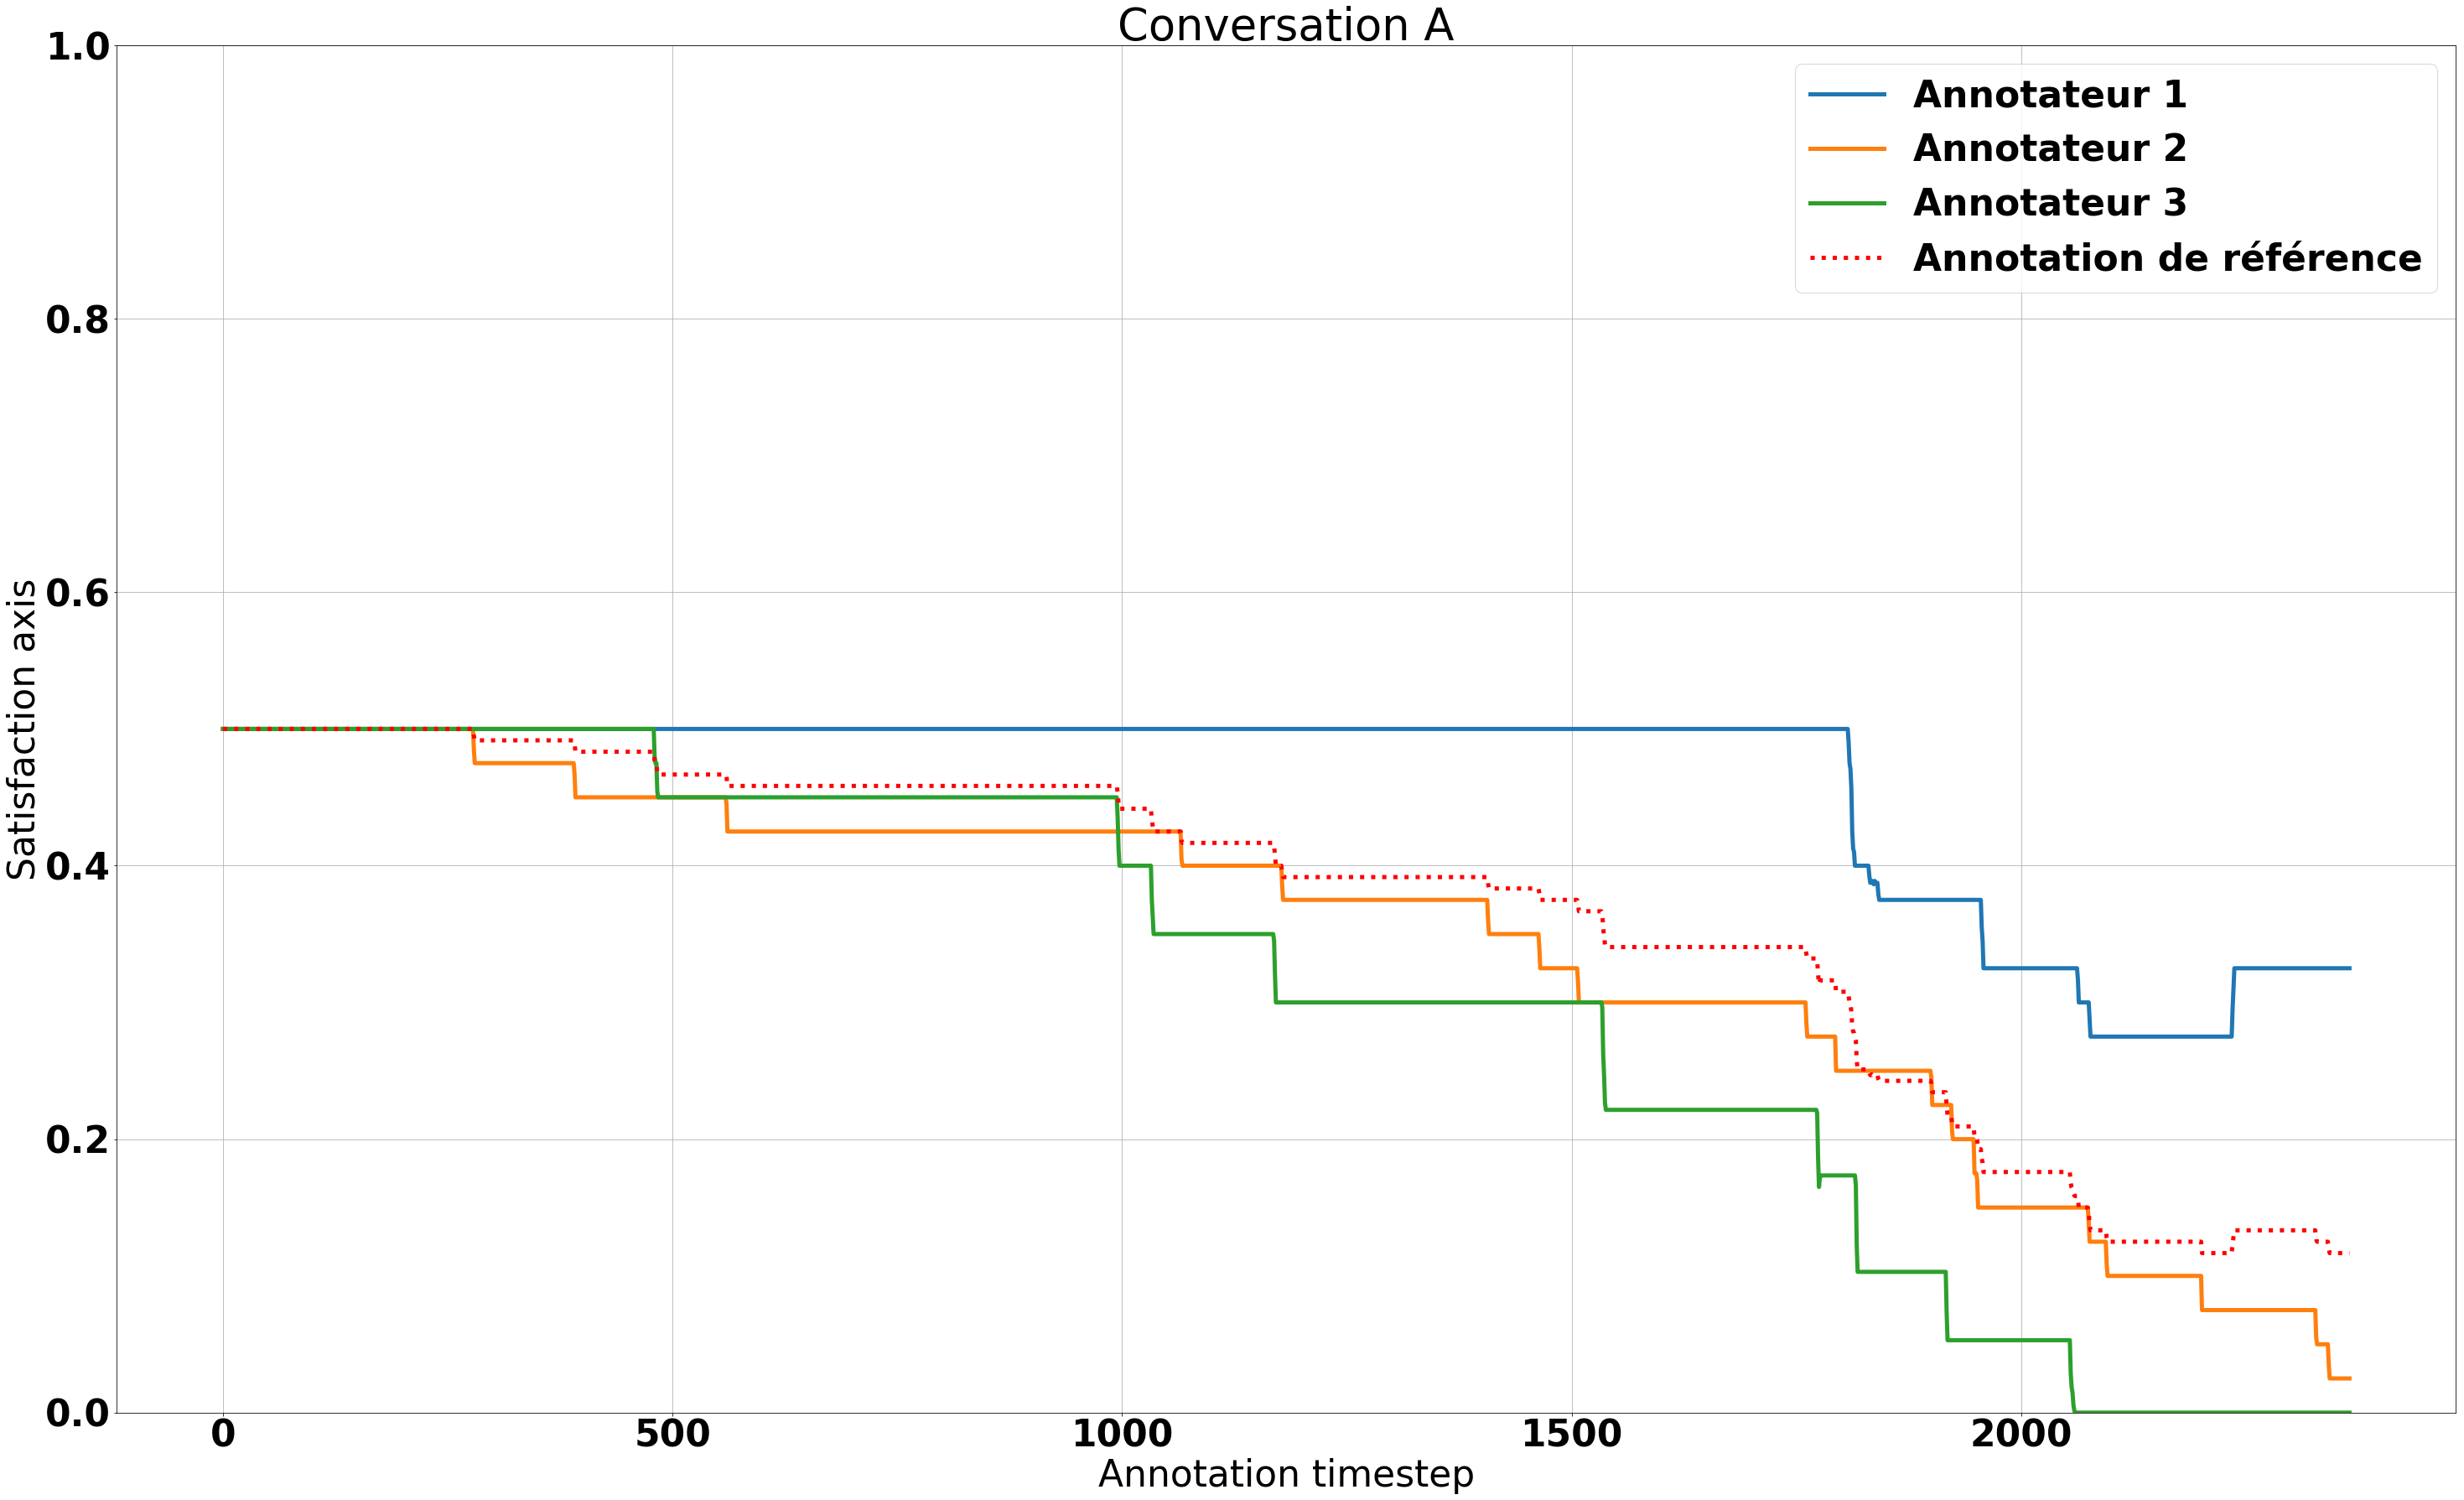
\includegraphics[width=15cm]{./Chapitre7/figures/annotTroisGold.png}
  \caption{Exemple d'annotation d'une conversation selon l'axe de satisfaction deja présenté chapitre 4. L'annotation de référence correspond à la courbe en pointillée}
  \label{fig:annotTroisGold}
\end{figure}


\begin{enumerate}
  \item Nous pouvons considérer les annotations de chaque annotateur indépendamment. En effet, nous pouvons partir du principe que la perception de l'émotion par chaque individu est légitime et peut être considérée comme une référence pour le système de détection.
  Ce positionnement va donc considérer que l'individu a plus de valeur que le groupe entier. Nous pouvons donc spécifier nos systèmes de reconnaissance pour reproduire le comportement d'un humain particulier.
  \item Nous pouvons également considérer la moyenne des annotations. En effet, faire la moyenne des annotations revient à généraliser ces dernières pour qu'elles soient plus en adéquation avec un ensemble d'individus et atténuer les perceptions qui s'écartent d'une normalité statistique. Ainsi, nous allons considérer que l'annotation de référence pour nos systèmes automatiques est la moyenne de l'avis de différentes personnes. Bien que ce procédé soit plus pertinent lorsque nous avons un nombre élevé d'annotateurs, il reste cohérent pour trois annotateurs et permet de généraliser nos systèmes de reconnaissance pour reproduire non pas le comportement d'un humain particulier mais d'un groupe d'humains.
\end{enumerate}

Au cours de la thèse, nous avons décidé, en adéquation avec les besoins industriels, de nous concentrer sur le deuxième positionnement, comme nous l'avons énoncé dans le chapitre~\ref{chapitre4}. Ce positionnement est également celui de nombreux travaux dans le domaine, notamment les travaux effectués sur les corpus RECOLA~\cite{Ringeval2013} et SEWA~\cite{SEWA}.

Cependant pour aller plus loin dans l'analyse du phénomène émotionnel, nous avons voulu explorer la possibilité d'utiliser les annotations de chacun afin de construire des systèmes de reconnaissance.

\subsection{Un modèle de reconnaissance par annotateur}
Si nous considérons que chaque annotateur donne une version légitime de l'émotion, nous pouvons choisir de construire trois modèles de reconnaissance en prenant les annotations des trois annotateurs. Pour ce faire, nous modifions la référence : au lieu d'entraîner un seul modèle sur la valeur moyenne des trois annotateurs, nous entraînons trois modèles différents par annotateur, dans lesquels les références correspondent aux valeurs uniques de cet annotateur.
Les prédictions de ces modèles sont évaluées en fonction des annotations individuelles (tableau~\ref{tab:ind_by_annotator}) ou de nos anciennes références définies comme la moyenne des trois annotations individuelles (tableau~\ref{tab:moy_by_annotator}).

Les colonnes AVG donnent les performances moyennes sur les trois modèles individuels. Les colonnes CV donnent le coefficient de variation (écart-type sur la moyenne) sur les trois modèles individuels. Diff1 est la différence relative entre linguistique et acoustique pris indépendamment et donne une idée du gain par annotateur.

\subsubsection{Annotations individuelles : }

\begin{table}[h]
    \centering
    \begin{tabular}{| l |cc| cc | cc | cc | cc |}\hline
     \textbf{Annotateurs} & \multicolumn{2}{c|}{$a_1$} & \multicolumn{2}{c|}{$a_2$}  &\multicolumn{2}{c|}{$a_3$} &\multicolumn{2}{c|}{AVG} & \multicolumn{2}{c|}{CV}\\
      & \textbf{Dev} &\textbf{Test} &\textbf{Dev}  &\textbf{Test} & \textbf{Dev} &\textbf{Test} & \textbf{Dev} &\textbf{Test} & \textbf{Dev} &\textbf{Test}\\ \hline

     Wav2Vec    & .834 & .734 & .731 & .785 & .841 & .597 & .802 & .705 & .077 & .138\\
     CamemBERT  & .898 & .877 & .833 & .834 & .900 & .804 & .877 & .838 & .043 & .044\\
     Diff1 (\%)           & 7.7 & 19.5 & 14.0 & 6.2 & 7.0 & 34.7 & - & - & - & -\\
     \hline
     Features              & .884 & .870 & .815 & .753 & .883 & \textbf{.834} & .861 & .819 & .046 & .073 \\
     \hline
     Modèle précoce    & .883 & .870 & \textbf{.855} & \textbf{.865} & .888 & .826 & .875 & \textbf{.854} & .020 & .028\\
     Modèle tardive     & .911 & .875 & .814 & .837 & \textbf{.921} & .799 & .882 & .837 & .067 & .045\\
     \hline
     Décision           & \textbf{.913} & \textbf{.882} & .840 & .849 & .916 & .793 & \textbf{.890} & .841 & .048 & .053 \\
     \hline

    \end{tabular}
    \caption{Résultats des systèmes de fusions pour chaque annotateur. Les modèles sont entraînés et évalués sur des annotations individuelles. AVG : moyenne sur les trois annotateurs. CV : coefficient de variation sur les trois annotateurs. Diff1 correspond à la différence absolue entre CamemBERT et Wav2Vec. La meilleure fusion est choisie sur le Dev.}
    \label{tab:ind_by_annotator}
\end{table}


Dans le tableau ~\ref{tab:ind_by_annotator}, nous pouvons remarquer que le coefficient de variation (CV), sans utiliser de fusions, est plus élevé avec les descripteurs acoustiques qu'avec les descripteurs linguistiques en particulier sur le Test. Plus précisément, concernant l'annotateur $a_3$, les performances de la modalité acoustique chutent sur le Test pour atteindre un score CCC de 0.597.
Ces résultats suggèrent que la prédiction de la satisfaction à partir des descripteurs acoustiques est plus sensible à la subjectivité de la tâche d'annotation qu'à partir des descripteurs linguistiques.

Notre hypothèse est que la variabilité dans l'espace acoustique est très diversifiée, et qu'une même réalisation acoustique peut être perçue avec des niveaux de satisfaction différents par le même annotateur, ce qui produit de moins bonnes performances sur la modalité acoustique.

En ce qui concerne la fusion des modalités, elle améliore les performances dans la plupart des configurations et les meilleures performances en moyenne sont atteintes avec la fusion modèle précoce avec un score de CCC de 0.854 sur l'ensemble de Test. L'amélioration sur le Test est la plus élevée avec l'annotateur $a_2$ ($+3.7$\% avec la fusion modèle précoce).
Cela peut s'expliquer par la très faible différence entre les performances obtenues sur des modalités acoustiques et linguistiques pour cet annotateur ($+6.2$\%), indiquant peut-être que les deux modalités portent des informations différentes pour cet annotateur spécifique.

A partir de ces résultats, nous émettons l'hypothèse qu'au niveau des annotateurs, les modalités acoustiques et linguistiques véhiculent des informations émotionnelles complémentaires. Cependant, si la partie linguistique est bien partagée entre les annotateurs, la perception de la partie acoustique semble assez individuelle.
Bien sûr, des expériences supplémentaires avec des annotations croisées sont nécessaires pour confirmer cette hypothèse.

\subsubsection{Annotations moyennes : }

\begin{table}[h]
    \centering
    \begin{tabular}{|l |cc| cc | cc | cc | cc|}\hline
     \textbf{Annotateurs} & \multicolumn{2}{c|}{$a_1$} & \multicolumn{2}{c|}{$a_2$}  &\multicolumn{2}{c|}{$a_3$} &\multicolumn{2}{c|}{AVG} & \multicolumn{2}{c|}{CV}\\
      & \textbf{Dev} &\textbf{Test} &\textbf{Dev}  &\textbf{Test} & \textbf{Dev} &\textbf{Test} & \textbf{Dev} &\textbf{Test}  & \textbf{Dev} &\textbf{Test}\\ \hline

     Wav2Vec    & .862 & .736 & .774 & .731 & .779 & .710 & .805 & .726 & .061 & .019\\
     CamemBERT  & .916 & .878 & .755 & .793 & .851 & .833 & .841 & .835 & .096 & .051\\
     Diff1 (\%)           & 6.3 & 19.3 & -2.5 & 8.5 & 9.2 & 17.3 & - & - & - & -\\
     \hline
     Features           & .896 & .845 & .741 & .688 & .868 & .861 & .835 & .798 & .099 & .120 \\
     \hline
     Modèle précoce     & .911 & .833 & \textbf{.809} & \textbf{.824} & \textbf{.879} & .856 & .866 & .838 & .060 & .020\\
     Modèle tardive      & .914 & \textbf{.899} & .763 & .784 & .844 & .841 & .840 & .841 & .090 & .068\\
     \hline
     Décision           & \textbf{.938} & .882 & .795 & .778 & .868 & \textbf{.874} & \textbf{.867} & \textbf{.845} & .082 & .069 \\
     \hline

    \end{tabular}
    \caption{Résultats des systèmes de fusions pour chaque annotateur. Les modèles sont entraînés sur des annotations individuelles et évalués sur les annotations moyennés de référence. AVG : moyenne sur les trois annotateurs. CV : coefficient de variation sur les trois annotateurs. Diff1 correspond à la différence absolue entre CamemBERT et Wav2Vec. La meilleure fusion est choisie sur le Dev.}
    \label{tab:by_annotator}
\end{table*}


En ce qui concerne les modèles individuels évalués avec des annotations moyennes (tableau ~\ref{tab:moy_by_annotator}), nous remarquons que l'annotateur $a_2$ a les performances les plus faibles lorsqu'il utilise uniquement des descripteurs linguistiques.
Le modèle construit sur cet annotateur atteint les performances les plus basses en utilisant n'importe quel type de fusion sur les ensembles de Développement et de Test.
Cette observation confirme ainsi l'importance des performances linguistiques qui ont un poids important dans l'évaluation générale de la satisfaction et la frustration quand on fusionne les modalités.
Ce résultat peut s'expliquer par le fait que parmi les trois annotateurs, nous avons montré que $a_2$ avait l'accord intra-annotateur le plus faible dans le chapitre~\ref{chapitre4}.

Nous pouvons également confirmer le fait que la fusion permet d'améliorer les performances par annotateur dans tous les cas.
Étonnamment, sur le Test, ces modèles fusionnés (CCC=0.884) surpassent même les modèles appris directement sur la référence traditionnelle (meilleur CCC=0.881). Néanmoins comme nous l'avons vu dans le chapitre~\ref{chapitre6}, une différence de 0.003 entre deux scores de CCC n'est pas vraiment significative.
La fusion modèle précoce a l'avantage d'avoir des performances moyennes plus élevées que CamemBERT et d'être le modèle le moins affecté par les annotations individuelles (CV = 0,020 sur l'ensemble de test).

De ces expériences, nous concluons que les approches de fusion semblent être plus robustes à la subjectivité de la tâche d'annotation. Nous avons constaté que la fusion modèle précoce était le meilleur compromis entre performance et robustesse.
Ces expérimentations remettent en question le processus d'évaluation largement utilisé qui compare les prédictions à la moyenne des annotations, en effet les valeurs moyennes n'ont pas de réalité perceptive, tandis que les valeurs individuelles en ont une. Il serait intéressant de mettre en place une étude du protocole d'évaluation sur d'autres corpus mais également de mener une étude perceptive sur les résultats de systèmes de reconnaissance ainsi construit.


\section{Expliquer la frustration dans les conversations}

\subsection{Première écoute humaine : que retire-t-on de l'acoustique ?}
Afin de mieux comprendre les données, nous avons arbitrairement choisi d'écouter 57 conversations choisies au hasard dans le corpus. Ces 57 conversations proviennent indépendamment des ensembles d'apprentissage, de développement et de test. Nous les avons classés dans deux catégories : bon ou mauvais, en fonction de leur score de reconnaissance issu de la classification sur la fusion des modalités. On considère comme bon, des scores supérieurs à $0.7$. Nous voulions mettre en lumière des facteurs explicatifs de la différence de score entre plusieurs conversations.

\begin{table}[h]
    \centering
    \begin{tabular}{|p{6cm}|c c c|}
         \hline
         Statistiques &Mauvais &Bon &Total \\
         \hline
         bruit &29 &22 &51 \\
         musique &7 &1 &8 \\
         conv. autre &11 &4 &15 \\
         silences &22 &11 &33 \\
         locuteur multiple &4 &1 &5 \\
         soupirs &7 &2 &9 \\
         rires &5 &0 &5 \\
         voix âgées &4 &0 &4 \\
         frustration manifeste &5 &20 &25 \\
         \hline
         femme &26 &11 &37 \\
         homme &9 &11 &20 \\
         \hline
         assurance &7 &12 &19 \\
         électricité/gaz &4 &3 &7 \\
         santé &2 &3 &5 \\
         voiture &3 &3 &6 \\
         autre &6 &13 &19 \\
         \hline
         variation annot faible &2 &26 &28 \\
         variation annot forte &20 &9 &29 \\
         \hline
    \end{tabular}
    \caption{Statistiques sur la présence d'événements retrouvés dans les 57 conversations écoutées.}
    \label{tab:ecouteHumaine}
\end{table}


Plusieurs phénomènes ont été observés sur ces conversations, qui sont indiqués dans le tableau~\ref{tab:ecouteHumaine}, mais nous n'avons pas trouvé un indicateur commun qui en émerge. En effet, ces conversations contiennent ou non du bruit, de la musique, plusieurs locuteurs, des rires, des voix âgées, des silences plutôt marqués (en début, milieu ou fin de conversations) et de la frustration manifeste (augmentation du débit de parole, du volume, moins de temps de silence, des injures,...). De plus, nous n'avons rien détecté qui permettrait de relier le sexe du locuteur ou les domaines d'activité dont sont issus les conversations et la variabilité des scores de prédiction.

En se concentrant sur des caractéristiques non linguistiques, nous n'avons pas trouvé de schéma clair et universel de la dimension de satisfaction avec ces observations.

\subsection{Études statistiques du contenu linguistique des conversations frustrées}

%\textcolor{red}{Pour cette partie je ne crois pas que le terme de "pic" soit adapté => pente de frustration ? et attention le rectangle jaune ne se voit pas bien => mettre en bleu ou noir ?}
Nous avons choisi d'extraire les contenus linguistiques correspondant aux pentes de frustration détectés par le modèle de reconnaissance. Pour cela, nous avons défini les pentes de frustration comme illustré dans la Figure~\ref{fig:pente} par le rectangle bleu. Concrètement, nous nous intéressons au coefficient de variation de la courbe tracée par la prédiction. Si on observe une variation décroissante de la prédiction supérieure à 0.1 point en 2 secondes, on considère que le segment de deux secondes correspond à un pente de frustration. Si on observe plusieurs pentes qui se chevauchent, on regroupe les segments sous la même annotation de pente.

\begin{figure}[h]
  \centering
  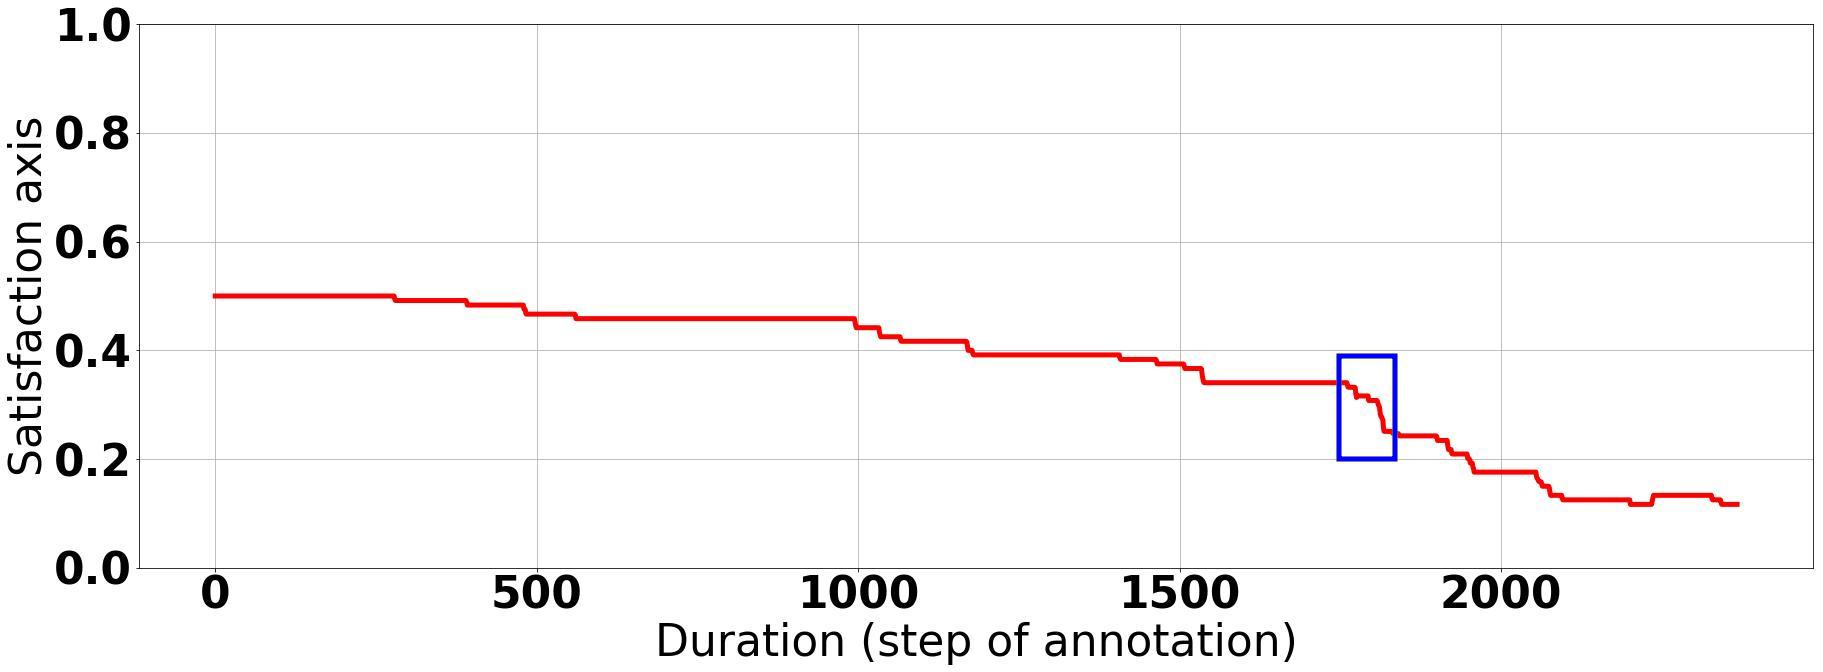
\includegraphics[width=15cm]{./Chapitre7/figures/pic.jpeg}
  \caption{Exemple de segment considéré comme une pente de frustration. Le rectangle bleu correspond au segment de pente de frustration.}
  \label{fig:pente}
\end{figure}


Une fois cet élément d'analyse mis en place, nous avons extrait les 166 transcriptions correspondant à ces pentes de frustration, en prenant du contexte gauche et droit à hauteur de deux secondes. Des exemples de segments ainsi récupérés sont indiqués dans le tableau~\ref{tab:phrasesPente}. On peut voir des mots issus de vocabulaire négatif comme \textit{perds mon temps} et \textit{avez fait l'erreur}, ainsi que des constructions spécifiques : des répétitions et une grande insistance sur le sujet avec des \textit{moi je} notamment.

\subsubsection{Utilisation de TF-IDF}

\begin{table}[h]
    \centering
    \begin{tabular}{|l|}
         \hline
         parce que d'abord je perds du temps alors moi je \\
         chacun son tour si vous voulez donc moi ce que je vous dis c'est que le véhicule \\
        ce que je me j'essaie de faire depuis au moins deux semaines \\
        vais faire appel à mon assistance juridique parce que \\
        vais tout supprimer et puis c'est tout \\
        juste pour dire en fait voilà il me faut ça point barre c'est ça \\
        putain mais visiblement c'est ça \\
        abonnement pour rien du tout \\
        c'est vous qui avez fait l'erreur donc je veux ma carte \\
        alors ça veut dire qu'il faut que je paie une blinde \\
        j'en ai vraiment besoin je comprends pas \\
         \hline
    \end{tabular}
    \caption{Exemple de transcription de segments considérés comme pente de frustration.}
    \label{tab:phrasesPente}
\end{table}


A partir de ces segments, nous avons conduit une analyse statistique. En utilisant TF-IDF, nous avons analysé les mots, les bi-mots et les tri-mots les plus pertinents. Nous avons ensuite utilisé le résultat de cette fonction pour construire des nuages de mots, illustrés dans la Figure~\ref{fig:nuageMot}. Comme nous pouvons le voir, il y a une forte représentation du \textit{je} dans les bi et tri-mots. On observe également beaucoup de tournures négatives (\textit{c'est pas, même pas, je sais pas, je suis pas, c'est pas possible}...) ainsi que des répétitions du mais. De plus, on retrouve des mots et des tournures a polarité négatives (\textit{un problème, gros soucis, déposer plainte, j'ai fait opposition, je suis débile, bêtise...}) et des références à des notions temporelles (\textit{dix jours, tous les mois, ce week-end...}). Néanmoins, si nous réalisons les mêmes opérations sur les autres segments, ne correspondant pas aux pentes de frustration, on peut retrouver une grande partie de ces observations.

\begin{figure}[h]
  \centering
  \begin{minipage}[b]{0.49\linewidth}
      \center
      \centerline{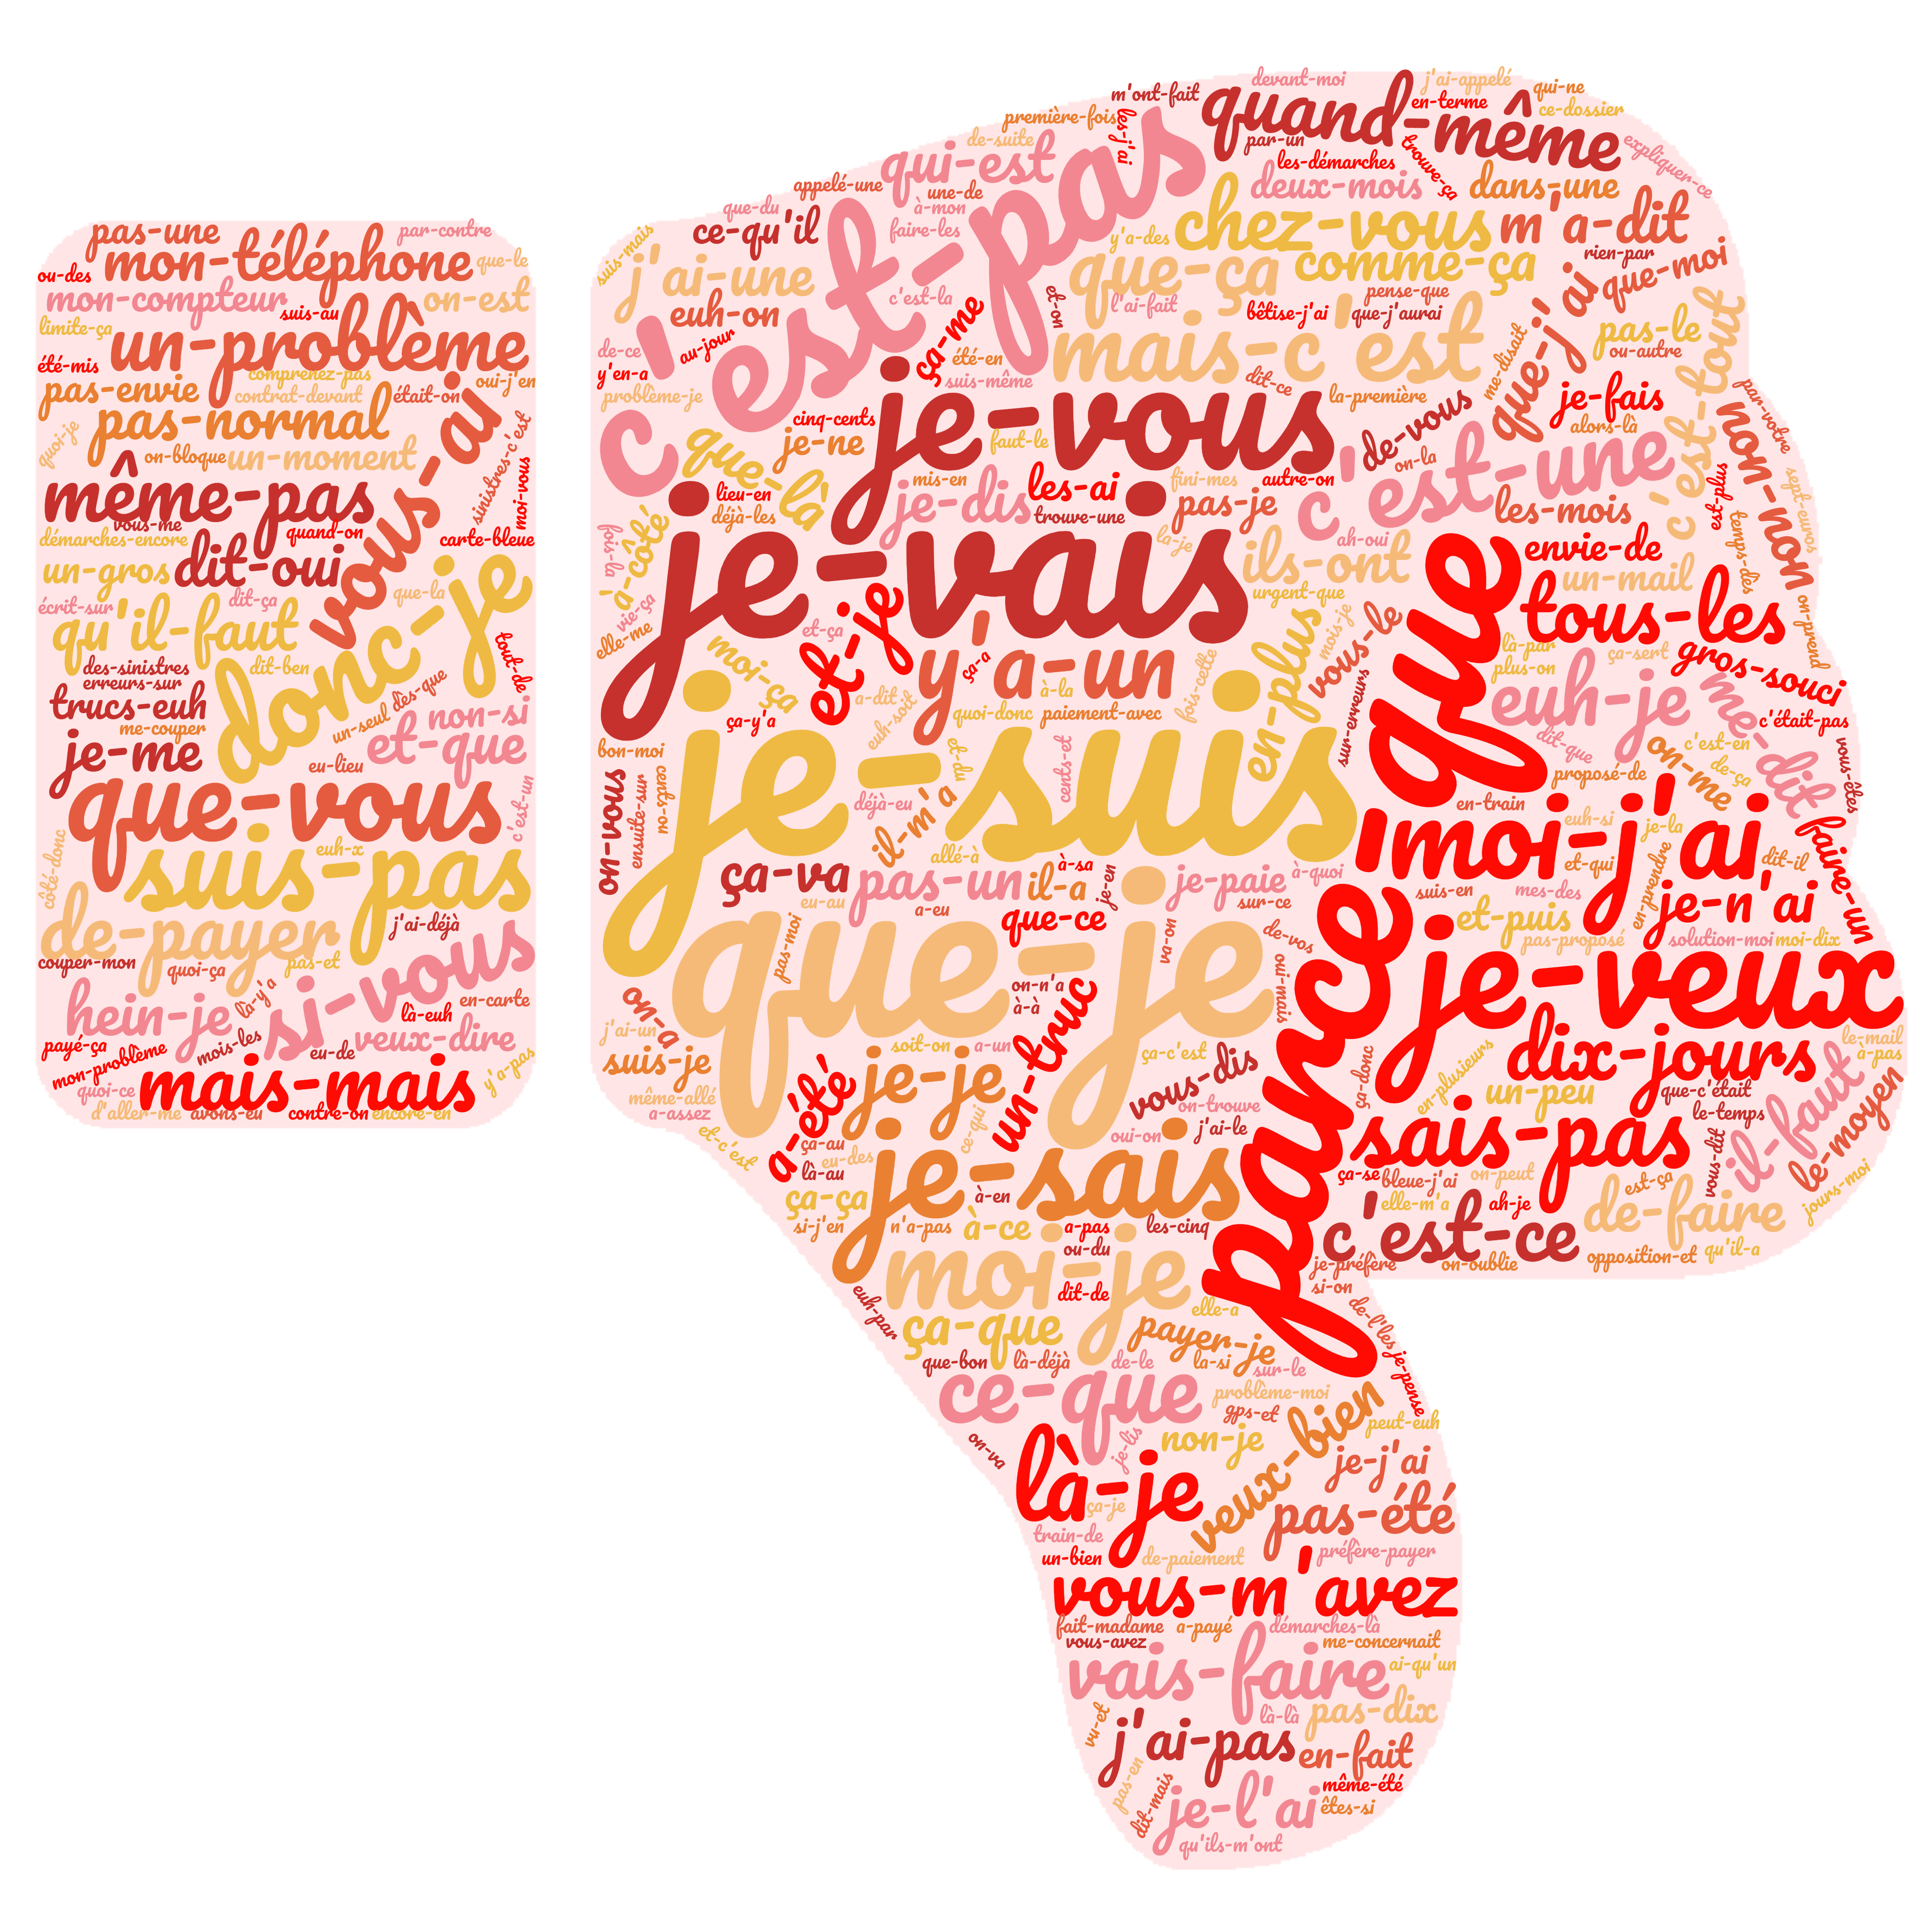
\includegraphics[width=8cm]{./Chapitre7/figures/bigram_pentu.png}}
  \end{minipage}
  \begin{minipage}[b]{0.49\linewidth}
      \center
      \centerline{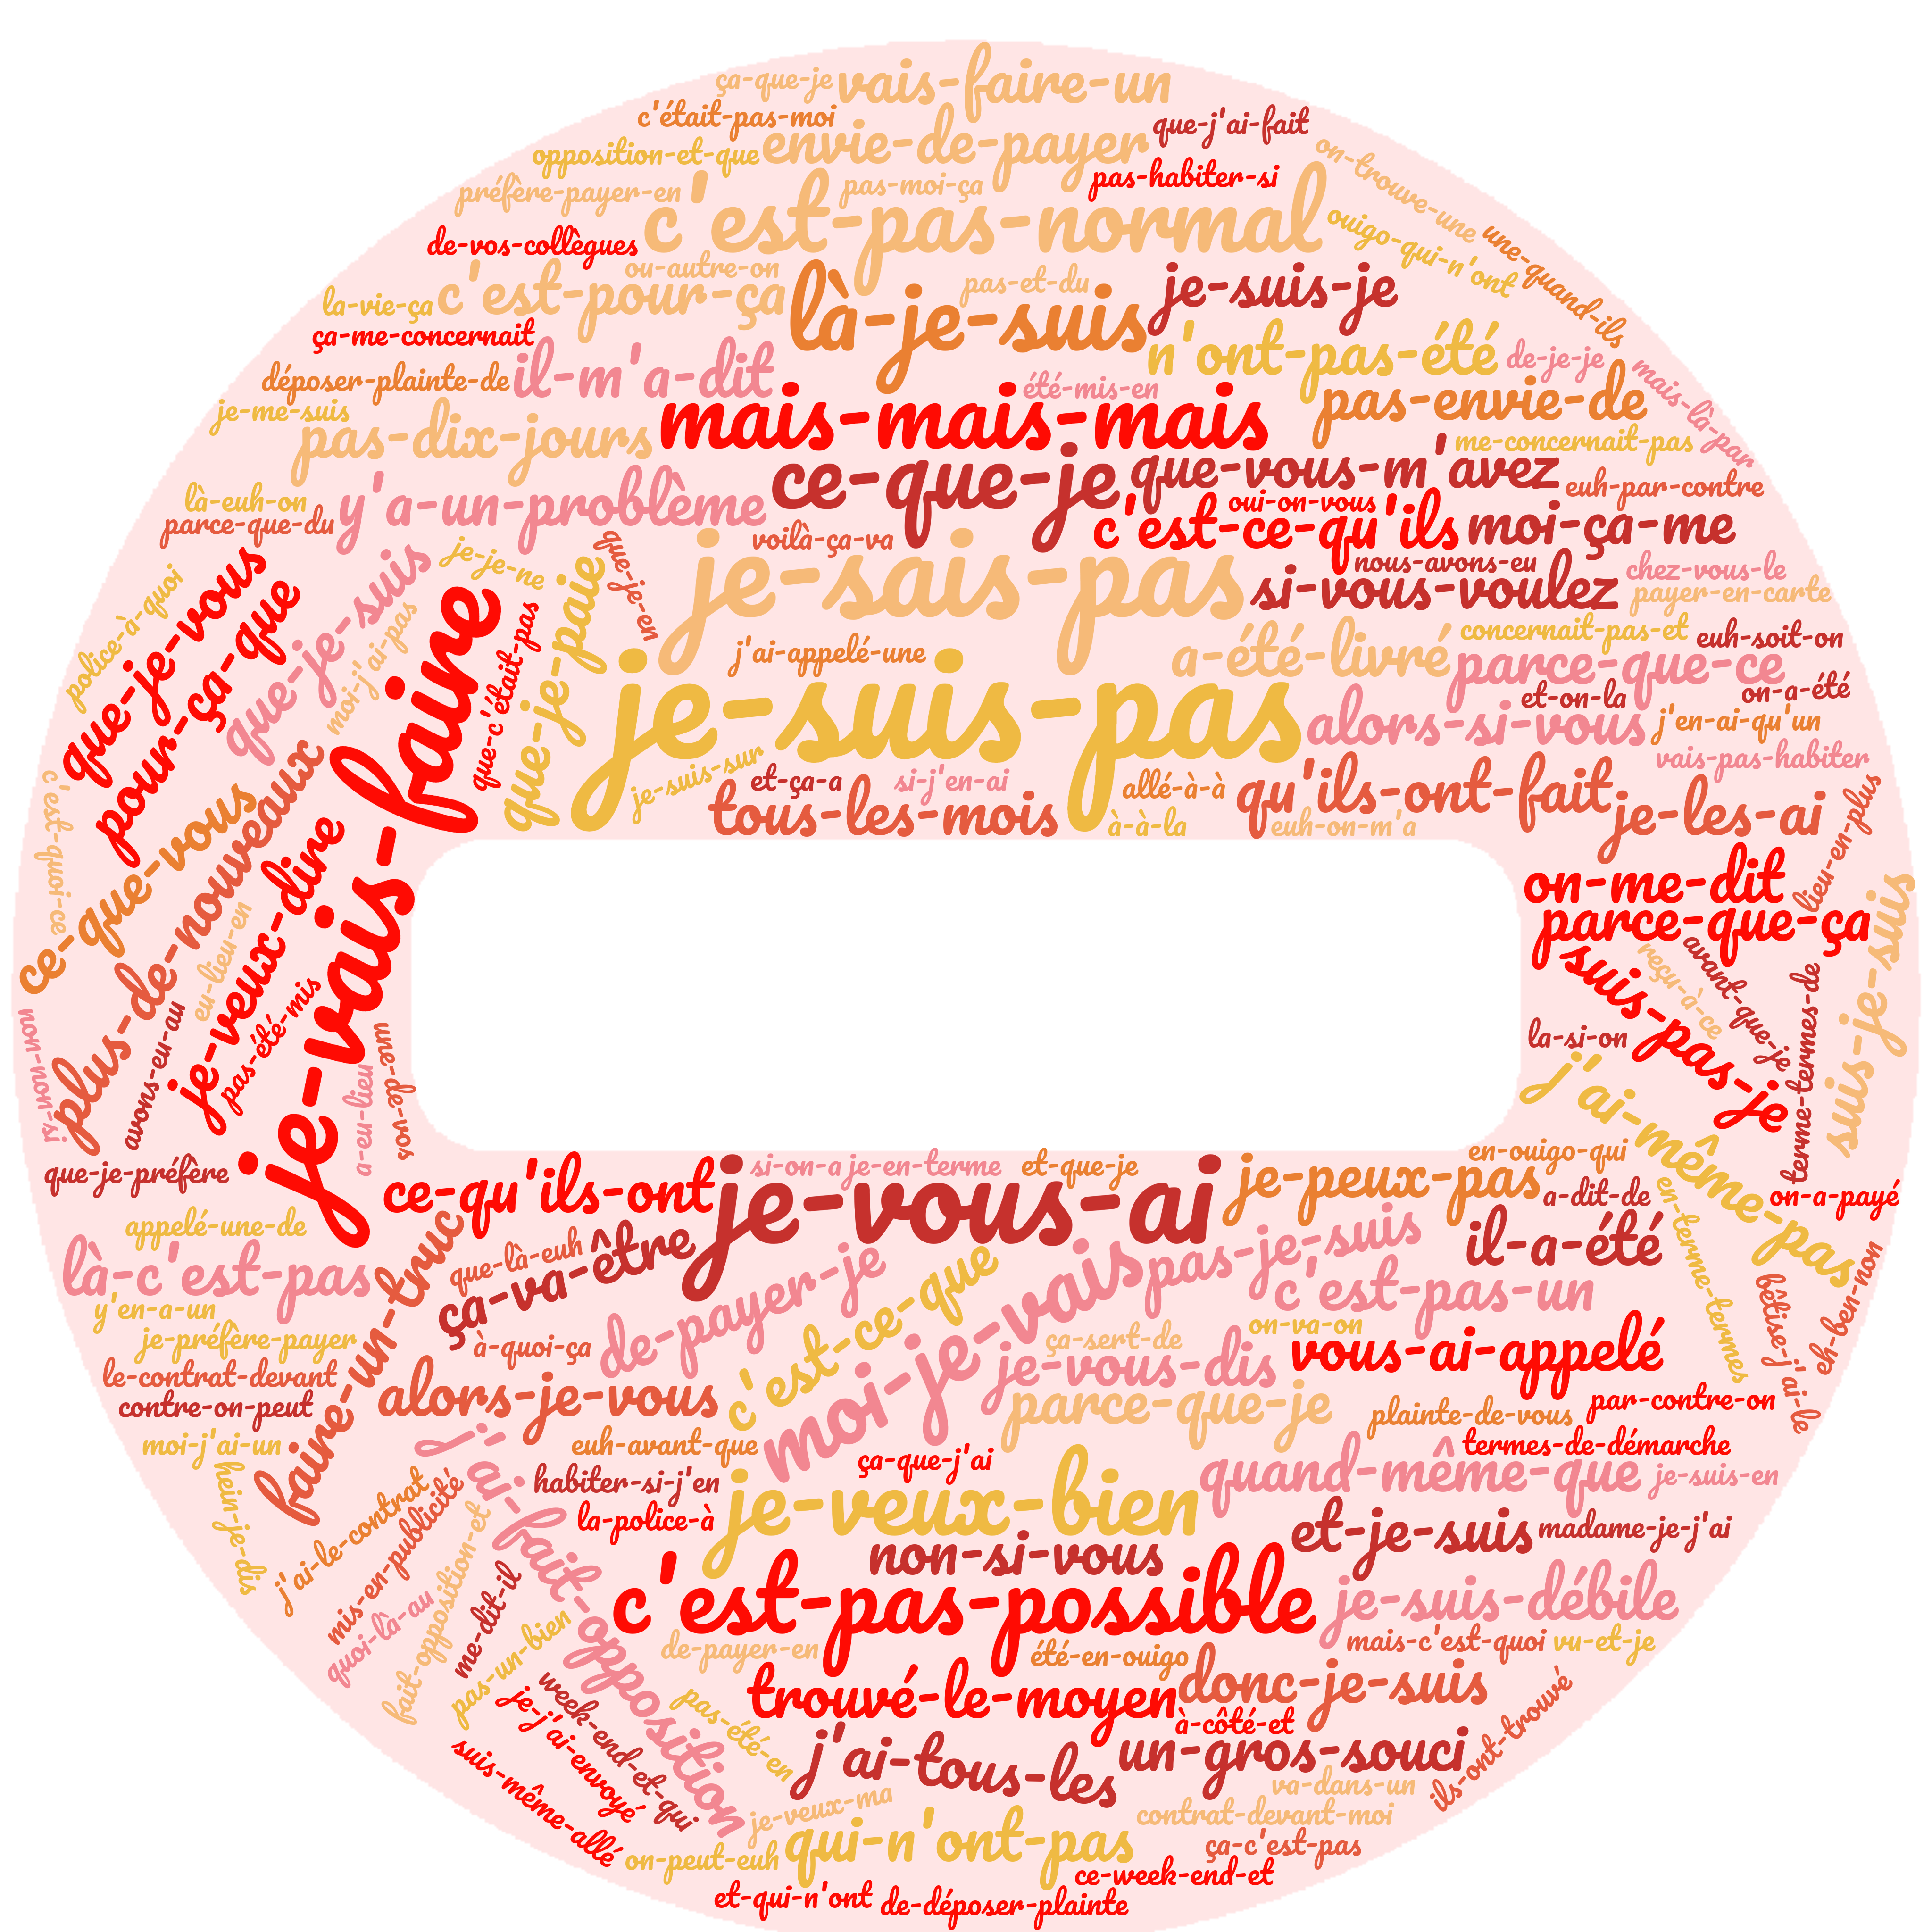
\includegraphics[width=8cm]{./Chapitre7/figures/trigram_pentu.png}}
  \end{minipage}
    \caption{Nuages de mots construits à partir des occurences de bi-mots (gauche) et tri-mots (droite) extraites des transcriptions des segments de pentes de frustration.}
    \label{fig:nuageMot}
\end{figure}


Nous avons également cherché au niveau de la syntaxe s'il y avait des schémas reconnaissables dans l'expression de la satisfaction. Pour cela, nous avons utilisé l’outil Macaon afin de faire un POS-tagging des segments. À partir du résultat de cette opération, nous pouvons extraire le rôle de chaque mot dans les segments mais nous n'arrivons pas à tirer des conclusions de ces observations. %(sujet, verbe, complément...). Nous avons alors utilisé un TF-IDF pour analyser les mots, bi-mots et tri-mots. Le tableau~\ref{tab:posPic} recense les différentes structures de segments que nous avons relevé. Nous n'arrivons pas à tirer des conclusions de ce classement.

%\begin{table}[h]
    \centering
    \begin{tabular}{|l|}
         \hline
          ROOT OBJ MOD SUJ OBJ P_OBJ OBJ ROOT ROOT ROOT
          ROOT DET ROOT ROOT SUJ OBJ COORD SUJ \textbf{DISFLINK} OBJ SUJ P_OBJ DEP_COORD COORD OBJ DET OBJ
          ROOT \textbf{DISFLINK}
          ROOT ROOT \textbf{DISFLINK} DET ROOT SUJ MOD MOD_REL MOD MOD
          \textbf{DISFLINK}
          ROOT OBJ OBJ MOD P_OBJ DET OBJ COORD P_OBJ DEP_COORD MOD MOD OBJ SUJ SUJ AUX OBJ
          ROOT ROOT SUJ OBJ MOD AFF OBJ P_OBJ DET OBJ COORD DET DEP_COORD
          ROOT ROOT SUJ OBJ SUJ ROOT SUJ ROOT OBJ OBJ OBJ DET OBJ ROOT OBJ ROOT
          ROOT MOD OBJ \textbf{DISFLINK} MOD OBJ AFF OBJ OBJ
          ROOT ROOT \textbf{DISFLINK} AFF DEP_COORD \textbf{DISFLINK}
          ROOT ROOT OBJ MOD OBJ MOD OBJ SUJ
          DET OBJ OBJ AFF OBJ OBJ OBJ \textbf{DISFLINK} \textbf{DISFLINK} MOD MOD ROOT
          AUX ROOT COORD DET SUJ AUX DEP_COORD P_OBJ OBJ
          ROOT \textbf{DISFLINK} OBJ ROOT MOD COORD DEP_COORD OBJ DET SUJ DEP_COORD
          ROOT OBJ OBJ ROOT DET OBJ MOD MOD ROOT
          ROOT MOD OBJ COORD ROOT DEP_COORD MOD
          ROOT \textbf{DISFLINK} \textbf{DISFLINK} ROOT
         \hline
    \end{tabular}
    \caption{Part-Of-Speech structure des segments correspondant aux pics de frustration.}
    \label{tab:posPic}
\end{table}


Comme nous n'arrivons pas à dégager clairement des caractéristiques communes à ces segments, nous avons pensé à utiliser le machine learning pour regrouper les segments en classes, et donc nous permettre de discerner les différences entre les classes. Ainsi nous pourrons peut-être décrire des marqueurs de frustration.

\subsubsection{Classification des segments de pente de frustration}
Comme nous n'avons pas de classes définies, nous avons fait le choix d'une classification non supervisée. Pour être cohérent avec le nombre limité de segments émotionnels (166), nous avons utilisé un classifieur de type kmeans avec k=3. Nous avons classifié les mots, bi-mots et tri-mots suivant ces 3 classes. Nous avons effectué une analyse en composantes principales afin de permettre la visualisation sur les deux premières composantes de nos classes, comme l'illustre la Figure~\ref{fig:kmeans}.

\begin{figure}[h]
  \centering
  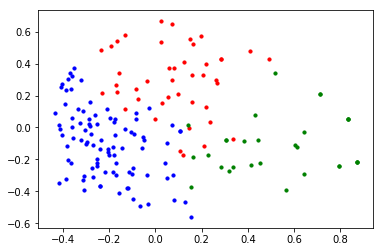
\includegraphics[width=8cm]{./Chapitre7/figures/datakmeans.png}
  \caption{Visualisation des données de segments émotionnels opérée par une pca, sur laquelle une classification de type kmeans (k=3) est effectuée.}
  \label{fig:kmeans}
\end{figure}


Nous avons ensuite utilisé des TF-IDF, dont nous avons expliqué le fonctionnement au chapitre~\ref{chapitre3}, sur les segments de chaque classe pour dégager des tendances. Les résultats sur les bi-mots et les tri-mots sont relatés dans le tableau~\ref{tab:kmeans}. Nous n'avons pas trouvé de caractéristiques bien saillantes dans ces classes qui permettraient de les dissocier à coup sûr. S'il fallait extrapoler, le premier cluster semble contenir des conversations en rapport avec les mutuelles; le deuxième cluster semble plutôt concerner des relances ou des clients qui ont déjà appelés; et le dernier cluster semble être peuplé de litiges de contrat (notamment de l'énergie).

\begin{table}[]
\centering
\begin{tabular}{|l|l|l|}
 \hline
 cluster 1 &cluster 2 &cluster 3 \\
 \hline
 au revoir 	& du tout 	&que je \\
 affiche bon 	& en fait 	& parce que \\
euh attendez 	& en ai 	& je vous \\
 eu lieu 	& qu on 	& je ai \\
la vie 	& je ai 	&ce que \\
 monsieur au 	& du coup 	& je suis \\
 et on 	&ai pas 	& si vous \\
 plus la 	&je comprends 	&que vous \\
 quatre fois 	& comprends pas 	&pas de \\
euh quatre 	&accord euh 	& et je \\
la fille 	&pas accord 	& ai envoyé \\
 je suis 	& est pas 	&moi ai \\
euh je 	& on fait 	& mais mais \\
il été 	& ils ont 	& ai appelé \\
 été livré 	& je vous 	&quand même \\
 personne ne 	&ont fait 	& je vais \\
 on sait 	&on est 	&vous comprenez \\
 ai appelé 	& fait madame 	&ai pas \\
 la rubrique 	& ai fait 	& suis je \\
lisez le 	& je peux 	&que ça \\
les choses 	&peux pas 	& est pas \\
mon billet 	& fait ça 	& je sais \\
 même allé 	& ce qu 	& donc je \\
 procès verbal 	&fait est 	& je veux \\
 la commande 	& ça fait 	&moi je \\
 faire les 	&ai ras 	&est ça \\
imprimer mon 	&ras le 	& vous voulez \\
 deux fois 	&le bol 	&que là \\
ai euh 	&un petit 	&que ai \\
 allé la 	& petit peu 	& alors que \\
annuler la 	&coup juste 	&je viens \\
assure votre 	&juste qu 	&élégant mais \\
 choses quoi 	&moi en 	&souci là \\
 de vous 	&est ça 	&mais bon \\
donc euh 	&pas du 	& viens appeler \\
 ils demandent 	& pour rien 	& là même \\
donc votre 	& rien du 	& je te \\
%  au revoir &0.027166	& du tout &0.030727	&que je &0.035652\\
%  affiche bon &0.014706	& en fait &0.028779	& parce que &0.032408\\
% euh attendez &0.014706	& en ai &0.027737	& je vous &0.026586\\
%  eu lieu &0.014706	& qu on &0.027021	& je ai &0.025469\\
% la vie &0.014706	& je ai &0.022723	&ce que &0.021531\\
%  monsieur au &0.013391	& du coup &0.019896	& je suis &0.020211\\
%  et on &0.012938	&ai pas &0.019834	& si vous &0.018290\\
%  plus la &0.010399	&je comprends &0.017689	&que vous &0.017569\\
%  quatre fois &0.010399	& comprends pas &0.017689	&pas de &0.016381\\
% euh quatre &0.010399	&accord euh &0.017678	& et je &0.016240\\
% la fille &0.010399	&pas accord &0.017678	& ai envoyé &0.016013\\
%  je suis &0.010307	& est pas &0.016991	&moi ai &0.014111\\
% euh je &0.010099	& on fait &0.016923	& mais mais &0.013664\\
% il été &0.009804	& ils ont &0.016289	& ai appelé &0.013534\\
%  été livré &0.009804	& je vous &0.016268	&quand même &0.013403\\
%  personne ne &0.009632	&ont fait &0.015485	& je vais &0.013385\\
%  on sait &0.008880	&on est &0.014932	&vous comprenez &0.013015\\
%  ai appelé &0.008864	& fait madame &0.014918	&ai pas &0.012487\\
%  la rubrique &0.008490	& ai fait &0.014918	& suis je &0.012430\\
% lisez le &0.008490	& je peux &0.014684	&que ça &0.012165\\
% les choses &0.008490	&peux pas &0.014684	& est pas &0.011947\\
% mon billet &0.008490	& fait ça &0.014575	& je sais &0.011900\\
%  même allé &0.008490	& ce qu &0.014359	& donc je &0.011601\\
%  procès verbal &0.008490	&fait est &0.014359	& je veux &0.011253\\
%  la commande &0.008490	& ça fait &0.014110	&moi je &0.011100\\
%  faire les &0.008490	&ai ras &0.014014	&est ça &0.011097\\
% imprimer mon &0.008490	&ras le &0.014014	& vous voulez &0.011065\\
%  deux fois &0.008490	&le bol &0.014014	&que là &0.010637\\
% ai euh &0.008490	&un petit &0.013868	&que ai &0.010344\\
%  allé la &0.008490	& petit peu &0.013868	& alors que &0.010280\\
% annuler la &0.008490	&coup juste &0.013549	&je viens &0.010248\\
% assure votre &0.008490	&juste qu &0.013549	&élégant mais &0.010248\\
%  choses quoi &0.008490	&moi en &0.013147	&souci là &0.010248\\
%  de vous &0.008490	&est ça &0.013095	&mais bon &0.010248\\
% donc euh &0.008490	&pas du &0.013023	& viens appeler &0.010248\\
%  ils demandent &0.008490	& pour rien &0.013023	& là même &0.010248\\
% donc votre &0.008490	& rien du &0.013023	& je te &0.009816\\
% euh ai &0.008490	& euh bon &0.013023	& ça va &0.009732\\
% euh donc &0.008490	& abonnement pour &0.013023	& vous ai &0.009701\\
% euh imprimer &0.008490	&tout euh &0.013023	&vais faire &0.009654\\
% relancer euh &0.008490	&comment on &0.012810	& ça ça &0.009608\\
%  hospitalisée deux &0.008490	&expliqué comment &0.012810	&alors si &0.009484\\
%  qui annuler &0.008490	&qui expliqué &0.012810	&même que &0.009442\\
%  être hospitalisée &0.008490	&deux jours &0.012431	&donc moi &0.009255\\
% verbal ils &0.008490	& pas envie &0.011997	&pas le &0.009107\\
%  vous relancer &0.008490	&envie de &0.011997	&pas me &0.009024\\
%  voilà euh &0.008490	&de payer &0.011997	&non si &0.008824\\
%  votre lisez &0.008490	& demain eu &0.011180	&et que &0.008768\\
%  de la &0.008458	& pas répondu &0.011180	& je fais &0.008755\\
% qu ils &0.008119	&moi du &0.011180	& il vous &0.008739\\
 \hline
\end{tabular}
\caption{Classification bi-mots des segments émotionnels correspondant aux pentes de frustration sur laquelle nous avons appliqué un TF-IDF.}
\label{tab:kmeans}
\end{table}


Nous avons donc fait le choix de nous tourner vers un linguiste, afin de collaborer sur l'analyse des transcriptions et retrouver des marqueurs humainement identifiables de la frustration.


\subsection{Analyses conduites par un linguiste}
Dans cette section, nous avons l'intention de fournir des éléments qui pourraient expliquer l'importance de la linguistique pour retrouver la satisfaction ou la frustration.
Cette analyse a été faite sur 13 conversations sélectionnées afin de couvrir différentes dynamiques de la dimension satisfaction : globalement plates, occurrences de frustration élevée (annotation de l'axe $<$ 0.4) et occurrences de satisfaction fortement décroissante (pente de frustration).
L'analyse a été effectuée à l'aide de la transcription automatique, de l'annotation de l'axe de satisfaction de référence et des balises correspondant à \textit{haute frustration} et \textit{pente de frustration}.

Notre hypothèse est que la parole frustrée comporte principalement  des accentuations des phénomènes oraux.
Par conséquent, nous avons relevé plus spécifiquement :
\begin{itemize}
    \item Quantité de disfluences,
    \item Hésitations, répétitions, bégaiements,
    \item Importance des auto-coupures définies comme \textit{les points où le flux d'énoncé est rompu}~\cite{Pallaud2019},
    \item Usage des interrogations et des négations,
    \item Preuves sémantiques de frustration ou au moins d'émotions négatives,
    \item Quantité de segments significatifs \textit{vs.} segments sémantiquement vides.
\end{itemize}

Sur la base de ces indices, l'analyse aboutit à différentes observations.
Il existe des marqueurs sémantiques de frustration dans les conversations telles que l'usage de la négation (\textit{ça ne m'amuse pas}, \textit{c'est inadmissible}) : des marqueurs forts (\textit{c'est gonflé}, \textit{putain de ...}) et des marqueurs faibles (\textit{quand même}, \textit{franchement}).
Il semble également que la quantité de segments significatifs, d'auto-ruptures et de disfluences, soit généralement corrélée à de fortes augmentations de frustration. La structure syntaxique des énoncés interrogatifs semble également corrélée à la frustration.

Dans un second temps, nous comptons aller plus loin dans cette analyse avec l'extraction automatique d'indices de la frustration.
Bien entendu, passer d'une extraction manuelle à une extraction automatisée en fonction du temps (avec un pas de 250~ms) implique de faire des choix dans la définition des indices.
%\textcolor{red}{Ici il faudrait préciser que c'est une extraction en fonction de temps avec un pas de 250ms ? dans le papier IEEE: "All the occurrences of features summarized in Table VII are synchronized in time together with the annotated satisfaction reference."}
En essayant de modéliser la quantité de segments significatifs, nous extrayons les balises POS à l'aide de MACAON~\cite{Nasr2011} directement à partir de transcriptions automatiques et calculons le nombre de verbes et de noms que l'on met en relation avec le temps.
Pour capturer les autres indices, nous avons décidé d'extraire automatiquement les sept caractéristiques mentionnées dans le tableau ~\ref{tab:ex_features}.

\begin{table}[]
    \centering
    \begin{tabular}{|l|c|}
      \hline
    \textbf{Caractéristiques} & \textbf{Nombre d'occurrences} \\\hline
    Répétition d'un mot (deg1)     & 26 \\
    Répétitions de deux mots (deg2) & 4\\
    Pauses dans le discours (\textit{euh, bah, hein, eh, etc.}) & 22\\
    Marqueurs forts (\textit{important, inquiet, scandaleux, etc.}) & 14\\
    Marqueurs faibles (\textit{quand même, franchement, etc.}) & 3\\
    Négations (\textit{pas, ne, n'}) & 30\\
    \textit{c'est} & 44\\ \hline
    nombre de mots dans \textit{lettre recommandée} & 1050 \\
    nombre de segment de parole dans \textit{lettre recommandée} & 152 \\ \hline
    \end{tabular}
    \caption{Sept caractéristiques et leur nombre d'occurrences permettent de modéliser les indices supposés être responsables de la frustration dans les conversations. Le nombre total de mots et de segments de parole de la conversation appelée \textit{lettre recommandée}, sont également indiqués.}
    \label{tab:ex_features}
\end{table}


L'idée n'est pas de fournir une analyse exhaustive sur l'ensemble des données mais de fournir quelques indices explicatifs. Nous nous concentrons ici sur l'analyse approfondie d'une seule conversation que nous appelons \textit{lettre recommandée}. Toutes les occurrences des caractéristiques résumées dans Table~\ref{tab:ex_features} sont synchronisées dans le temps avec la référence de satisfaction annotée.

\begin{figure}
    \centering
    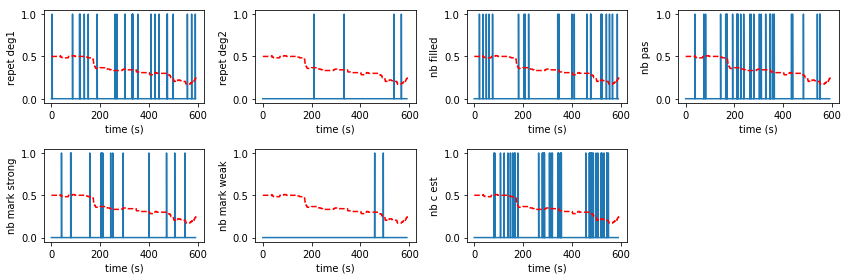
\includegraphics[width=\textwidth]{./Chapitre7/figures/ex_dynamic.png}
    \caption{Analyse dynamique de la frustration de la conversation appelée \textit{lettre certifiée}. Le nombre d'occurrences des sept caractéristiques linguistiques est tracé par rapport au temps. La référence de l'axe de satisfaction est représentée par la ligne en pointillée rouge.}
    \label{fig:ex_dynamic}
\end{figure}


Les quantités de verbes et de noms ne donnent pas d'information pertinente et ne sont pas représentées ici. L'analyse linguistique dynamique est présentée sur la Fig.~\ref{fig:ex_dynamic}. La conversation \textit{lettre recommandée} a été annotée avec une forte baisse de satisfaction avant 200~sec. La transcription automatique obtenue juste avant cette chute est donnée dans le Tableau~\ref{tab:ex_transcription}. Juste avant la chute, les occurrences de répétition de mots simples et de \textit{c'est} sont importantes, alors qu'après la chute, le nombre de pauses remplies par des interjections (\textit{euh, bah, hein, eh}, etc...) et de marqueur de négation (\textit{pas}) augmente. On remarque également qu'un marqueur fort (\textit{réclamation}) se produit juste avant la chute, signifiant probablement que ce mot spécifique induit chez l'annotateur la perception d'une frustration notable.

\begin{table}[h]
    \centering
    \begin{tabular}{|p{0.80\textwidth}|}
      \hline
    - \textit{voilà} et \underline{la deuxième lettre}  // c'est pareil \textit{mais bon} \underline{cette lettre}  // \underline{elle} est où maintenant… pas comprendre pourquoi on n'a pas retiré \underline{la lettre}... \underline{la deuxième lettre}  // c'est pareil \textit{mais} \underline{elle} venait d'où  // \underline{cette lettre}... c’était \underline{qui}  // \underline{qui} a envoyé \underline{cette lettre}... parce que c'est important  // on est une société  // nous… \underline{quand on sait pas qui c'est} // ... \underline{comment on peut savoir qui c'est} \textit{ouais mais} \underline{\textbf{ça va pas du tout}} \textit{hein} \underline{\textbf{ça va pas du tout}}  // \underline{ça}
    \\ \hline
    \end{tabular}
    \caption{Extrait (137 - 166~sec.) de la conversation \textit{lettre certifiée}. Disfluences: \textit{italic}; Hesitations, bégaiements: \underline{underline}; Traces Semantiques de la frustration: \textbf{bold}; auto-coupures: //}
    \label{tab:ex_transcription}
\end{table}


Dans le corpus AlloSat, l'information émotionnelle extraite semble résider davantage dans les mots que dans le contenu prosodique et acoustique. Dans ces données, l'expression de la frustration est principalement liée à l'accentuation des phénomènes oraux : le contenu sémantique et surtout les auto-coupures, les disfluences, les hésitations et les répétitions.

\section{Considération du genre}
Nous avons voulu conduire une analyse genrée des échanges entre les clients et les conseillers. En effet, nous voulons voir si le genre a un impact sur la frustration et son expression dans notre corpus. Pour ce faire, nous avons extrait les paires clients-conseillers dont nous avions les informations, soit 81 conversations sur les 303. En effet, le corpus ne comportant pas de données sur le conseiller, il s'agit de données confidentielles soumises à la RGDP, qui explique que la plupart des métadonnées des conversations ne sont pas conservées par l'entreprise.

\begin{table}[]
\centering
\begin{tabular}{|l l|l|l|}
 \hline
 Client	&Conseiller	&Nombre de conversation	&Pente de frustration présent \\
 \hline
femme	&femme	&38	&9	\\
homme	&homme	&5	&0	\\
femme	&homme	&17	&5	\\
homme	&femme	&21	&7	\\
 \hline
\end{tabular}
\caption{Présence de pentes de frustration en fonction du genre de la pair d'interlocuteur.}
\label{tab:genre}
\end{table}


Nous avons voulu mettre l'accent sur les conversations portant des pentes de frustration tel que définis dans ce chapitre. Comme nous pouvons le voir dans le tableau~\ref{tab:genre}, il n'y a pas assez de données pour donner une quelconque conclusion significative. Dans la Figure~\ref{fig:genre}, nous avons l'impression que les hommes sont plus énervés quand ils ont une femme en tant qu'interlocutrice et que la frustration est plus présente sur les pairzs hétérogènes.

\begin{figure}[h]
  \centering
  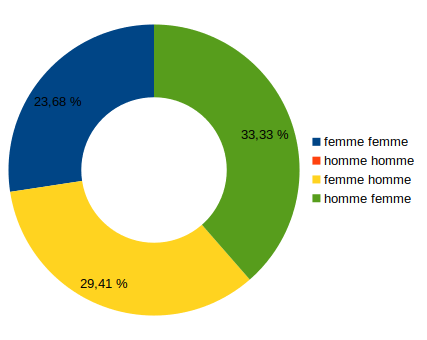
\includegraphics[width=10cm]{./Chapitre7/figures/genre.png}
  \caption{Visualisation du pourcentage de conversations contenant des pics de frustration en fonction du genre de la pair d'interlocuteurs. Le couple homme-homme n'apparait pas puisqu'il n'y a pas de conversations avec un pic de frustration pour cette pair d'interlocuteurs dans les 81 conversations considérées.}
  \label{fig:genre}
\end{figure}


 Il serait intéressant de conduire une étude plus large sur l'impact du genre des interlocuteurs sur l'expression de la frustration.

\section{Conclusion}
Dans ce dernier chapitre de contribution, nous avons souhaité prendre du recul sur nos travaux et expliquer nos résultats. Nous avons tout d'abord discuté de l'utilisation d'une annotation moyennée comme référence à nos systèmes de reconnaissance et plus largement de la pertinence de ce protocole qui est très largement adopté au sein de la communauté scientifique pour les tâches ayant une part non négligeable de subjectivité. Nous nous sommes ensuite concentrés sur la modalité linguistique de notre corpus, à savoir les transcriptions automatiques des conversations, et nous avons essayé de mettre en lumière les facteurs expliquant la très bonne performance des systèmes de reconnaissance appris à partir du texte. Enfin nous avons considéré rapidement l'impact du genre sur la frustration.

Nous pouvons conclure qu'il est difficile de statuer sur des marqueurs linguistiques de la frustration. En effet, en tant qu'humain, nous ressentons bien cette frustration dans le texte, sans pour autant pouvoir définir des marqueurs clairs et universels de cette émotion. Nous pouvons néanmoins souligner la présence des disfluences, des auto-coupures et des bégaiements comme des marqueurs pouvant alerter sur une potentielle frustration.
